\documentclass[a4paper, 12pt]{article}

\usepackage[english, russian]{babel}
\usepackage[T2A]{fontenc}
\usepackage[utf8]{inputenc}
\usepackage{mathtext}
\usepackage{amsfonts}
\usepackage{ amssymb }
\usepackage{amsmath}
\usepackage{graphics}
\usepackage{graphicx}
\usepackage{wrapfig}
\usepackage{geometry}
\usepackage{float}
\geometry{
    a4paper,
    total={170mm, 257mm},
    left=20mm,
top=10mm}

\title{Лабораторная работа 3.4.2. Закон Кюри-Вейсса}
\author{Сидорчук Максим, Б01-204}
\date{\today}

\begin{document}
\maketitle

\section*{Краткая теория}
В данной лабораторной работе предлагается проверить закон Кюри-Вейсса: при температуре выше температуры Кюри:
\[\chi \sim \frac{1}{T - \theta_P}\]
$\theta_P$ - парамагнитная точка Кюри.\\
Исследуемый материал будет помещен в катушку индуктивности, из-за чего её индуктивность будет меняться с температурой:
\[L - L_0 \sim \mu - 1 = \chi\]
Изменение индуктивности будем наблюдать с помощью изменения периода колебаний: $\tau = 2\pi\sqrt{LC}$, поэтому
\[L - L_0 \sim \tau^2 - \tau_0^2 \ \rightarrow \ \chi \sim \tau^2 - \tau_0^2 \ \ \rightarrow \ \frac{1}{\tau^2 - \tau_0^2} \sim T - \theta_P\]
Здесь $L_0$ и $\tau_0$ - индуктивность и период колебаний без образца в катушке соответственно.
\section*{Экспериментальная установка}

Исследуемый ферромагнитный образец (гадолиний) расположен внутри пустотелой катушки самоиндукции, которая служит индуктивностью колебательного контура, входящего в состав $L C$ -автогенератора.

\begin{center}
    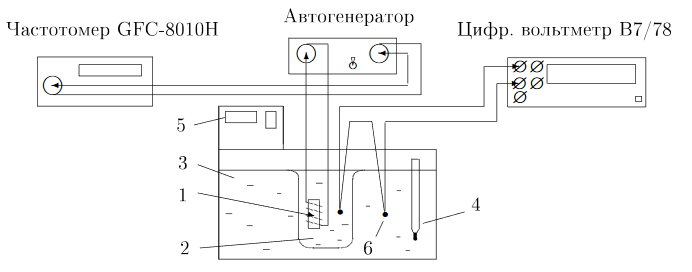
\includegraphics[width=0.8\textwidth]{1.png}
    \label{pic1}
\end{center}
Катушка 1 с образцом помещена в стеклянный сосуд 2, залитый трансформаторным маслом. Масло предохраняет образец от окисления и способствует ухудшению электрического контакта между отдельными частичками образца. Кроме того, оно улучшает тепловой контакт между образцом и рабочей жидкостью 3 в термостате. Ртутный термометр 4 используется для приближённой оценки температуры.\\
При изменении температуры меняется магнитная восприимчивость образца $\chi,$ а следовательно, самоиндукция катушки и период колебаний $\tau$ автогенератора. Для измерения периода используется частотомер. \\
Измерения проводятся в интервале температур от $14^{\circ} \mathrm{C}$ до $40^{\circ} \mathrm{C} .$
Температура исследуемого образца всегда несколько отличается от температуры дистиллированной воды в сосуде. Эта разность температур фиксируется термопарой, чувствительность которой $\mathrm{K}=24\frac{\text{град}}{\text{мВ}}$. ЭДС термопары измеряется цифровым вольтметром.


\section* {Результаты измерений и их обработка}
Полученные значения $\tau$ при разных температурах записаны в таблице. Показания цифрового вольтметра изменялись достаточно сильно, поэтому примем их погрешность $\sigma_U = 0,002$ мВ, что в измерении температуры даст погрешность $0,05^{\circ} C$. Вместе с погрешностью измерения температуры в термостате $0,05^{\circ} C$ получаем погрешность $0,07^{\circ} C$ в измерении температуры образца.\\
Период колебаний без образца внутри катушки: $\tau_0 = 6.9092$ мкс.
\begin{table}[h!]
    \centering
    \begin{tabular}{|c|c|c|c|}
        \hline
        $t, ^{\circ}C$ & $\Delta U$, мВ & $\tau$, мкс \\ \hline
		14.11 &	-11 &	7.9212 \\\hline
		16.11 &	-9 &	7.8567 \\\hline
		18.11 &	-12 &	7.758 \\\hline
		20.11 &	-5 &	7.5611 \\\hline
		22.8 &	-9 &	7.3836 \\\hline
		24.07 &	-14 &	7.2207 \\\hline
		26.09 &	-7 &	7.1263 \\\hline
		28.09 &	-4 &	7.0831 \\\hline
		30.08 &	-5 &	7.0578 \\\hline
		32.06 &	-11 &	7.0423 \\\hline
		34.05 &	-12 &	7.0285 \\\hline
		36.04 &	-16 &	7.0185 \\\hline
		38.06 &	-9 &	7.009 \\\hline
		40.04 &	-10 &	7.0033 \\\hline
    \end{tabular}
    \caption{Значения периода колебаний в зависимости от температуры образца}
\end{table}

По этим данным построим график $\frac{1}{\tau^2 - \tau_0^2} = f(T)$. Аппроксимируем прямой часть графика, начиная с четвертого значения. Получили прямую $y \approx 0,348x - 5,96$. Тогда она пересечет ось абсцисс в точке $\theta_P = (17,12 \pm 1,44) ^{\circ}C $
Точку Кюри по графику определить достаточно сложно, если аппроксимировать первые несколько значений прямой, то точка Кюри будет примерно $\theta = 5,35^{\circ}C$.
\begin{figure}[h!]
    \centering
    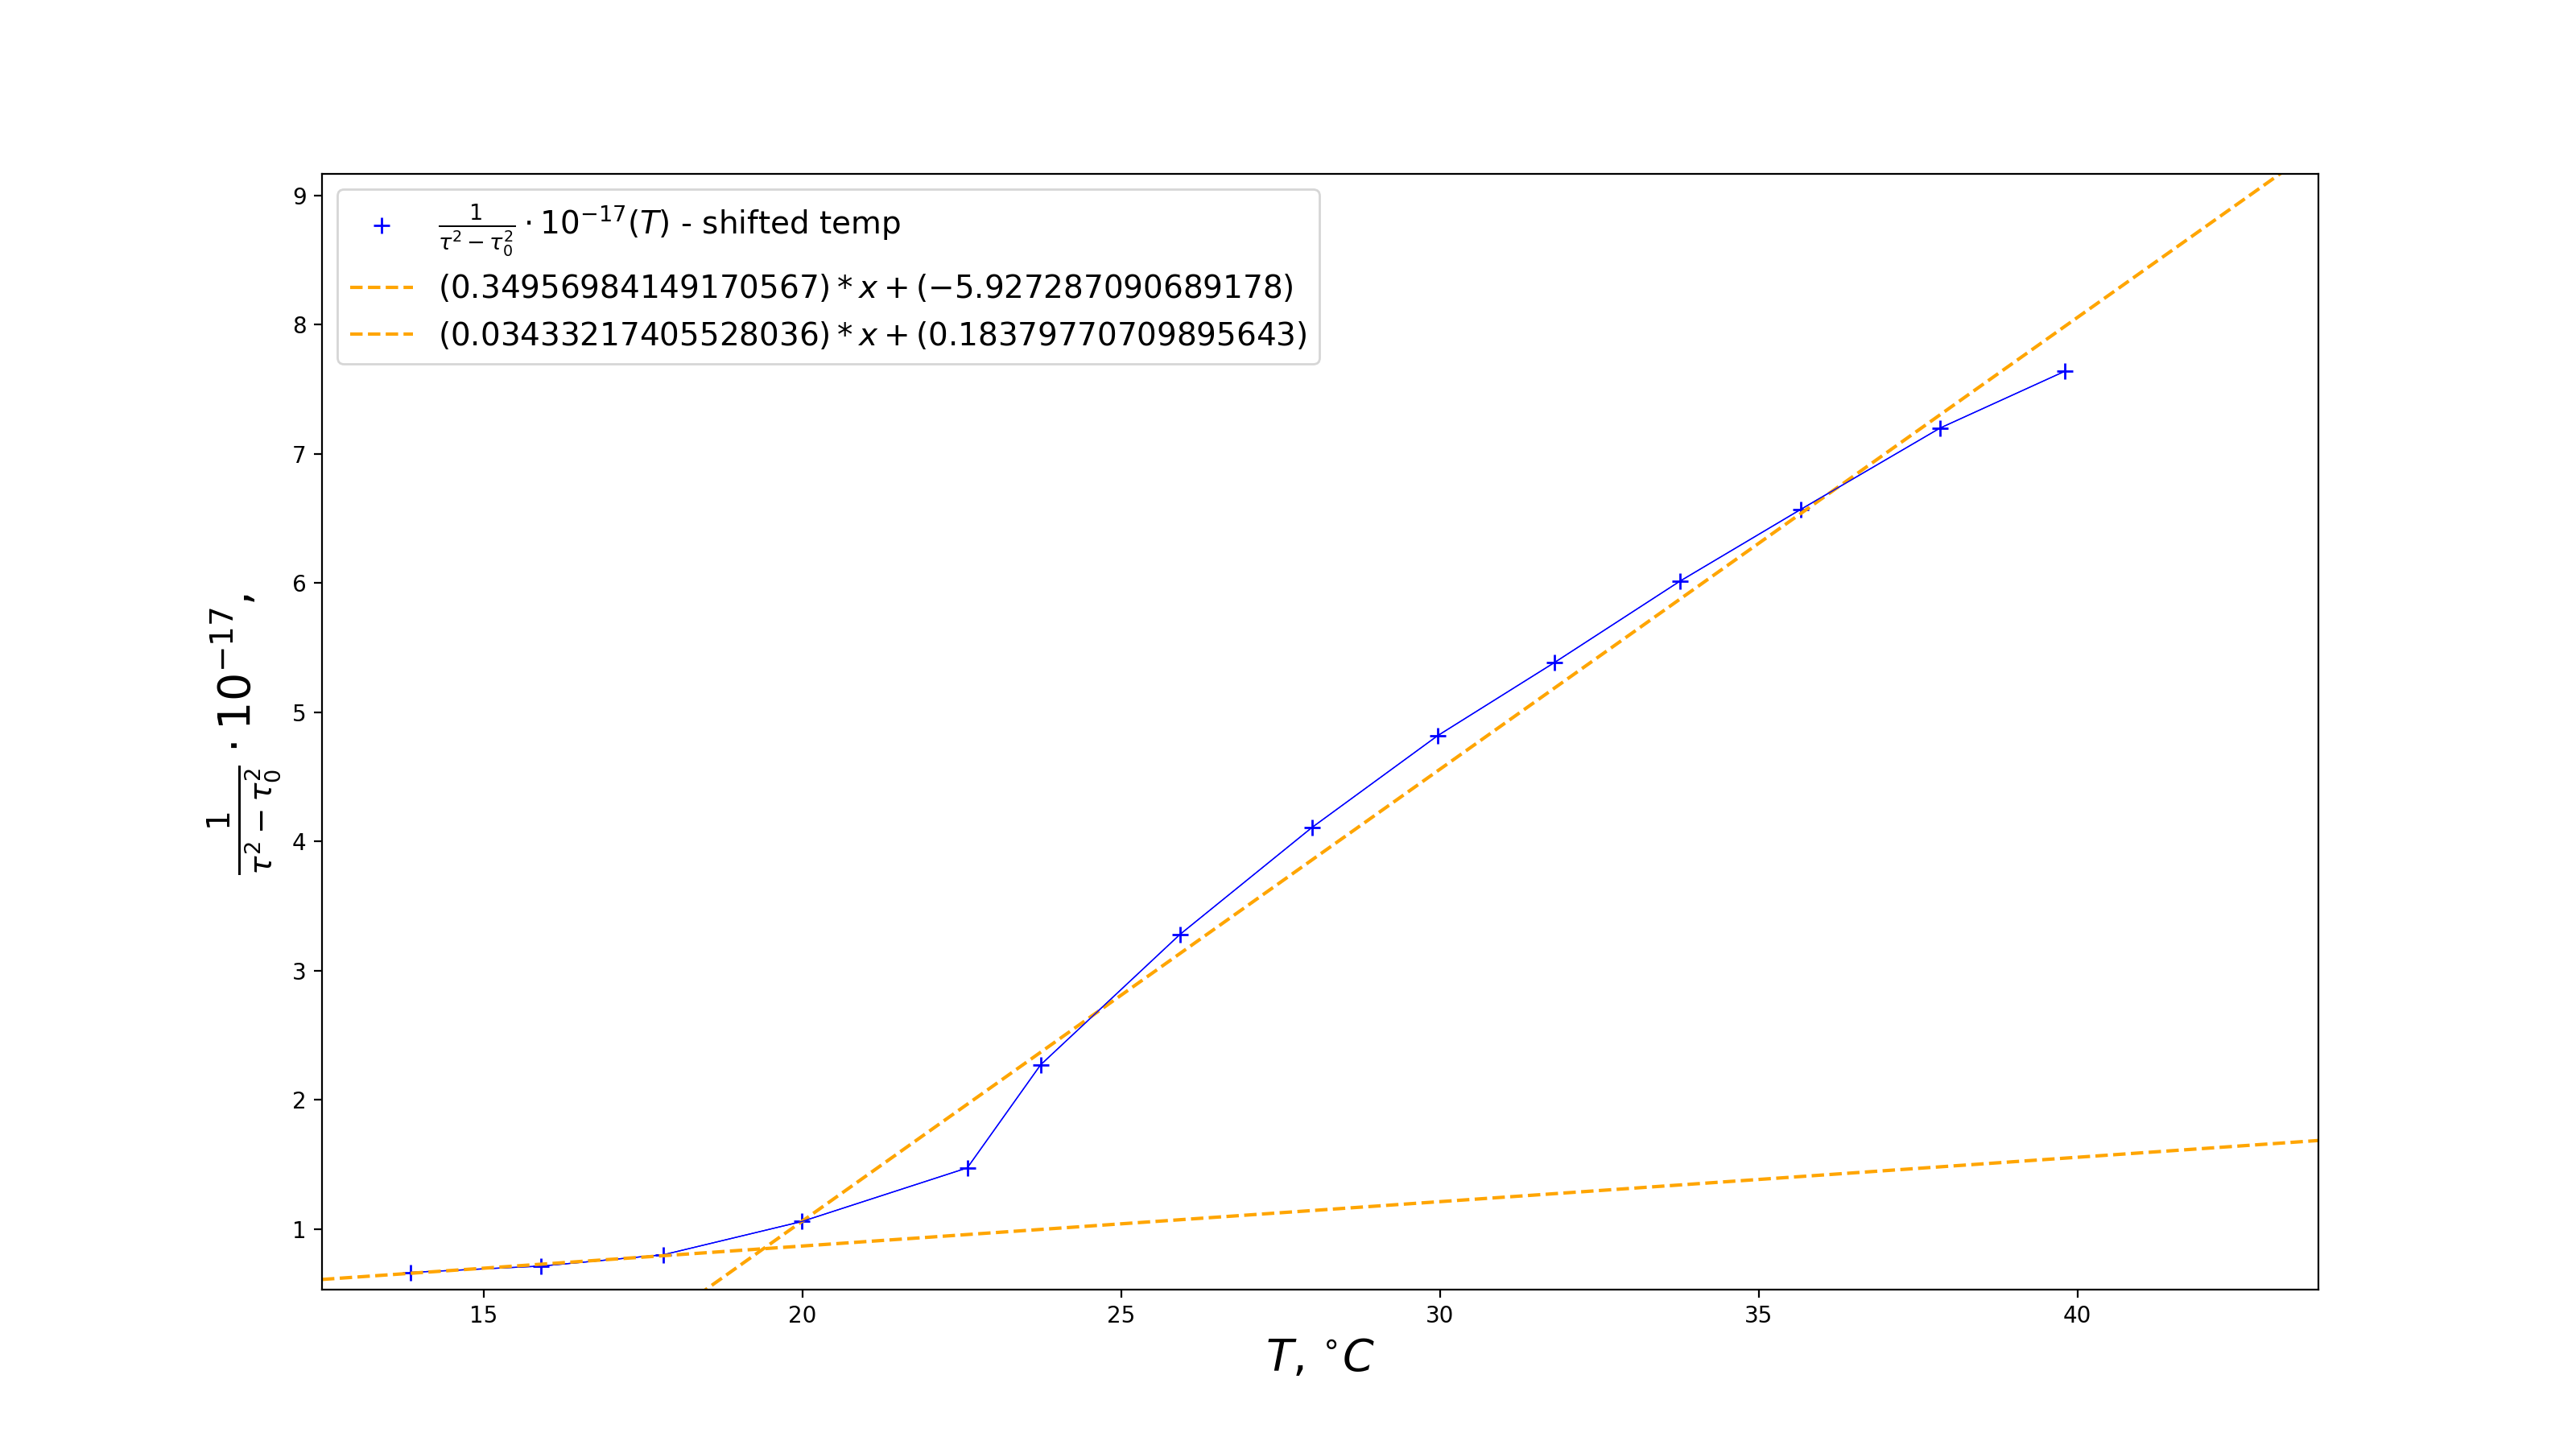
\includegraphics[width = \textwidth]{lol.png}
    \caption{Зависимость $\frac{1}{\tau^2 - \tau_0^2} = f(T)$}
\end{figure}
\section*{Выводы}
В данной лабораторной работе мы проверили выполнимость закона Кюри-Вейсса, получив график зависимости $\frac{1}{\tau^2 - \tau_0^2} = f(T)$. Зависимость совпадает с теоретической по характеру, но значения точки Кюри и парамагнитной температуры Кюри достаточно сильно отличаются от теоретических: $\theta_{th} = 20,2^{\circ}C, \ \ \theta_{P_{th}} > \theta_{th}$. Различия связаны, прежде всего, с способом получения данных: график построен в координатах $\frac{1}{\tau^2 - \tau_0^2} = f(T)$, а $\frac{1}{\tau^2 - \tau_0^2} \sim \frac{1}{\chi}$, то есть строго равенства нет, есть только пропорциональность, а парамагнитная температура Кюри определяется из графика $\frac{1}{\chi}(T)$. Температура Кюри определялась экстраполяцией прямой на нелинейной зависимости, для которой мало точек, поэтому значения неточные.
\end{document}
